\chapter{The gadolinium phase of Super-Kamiokande}
\label{cha:skgd}

As studied in the previous chapter, the typical total cross-section for an accelerator neutrino \mbox{($\sim1$\,GeV)} %
is of the order of \np{e-38}\,cm\tapi{2} and for a solar neutrino ($\lesssim10$\,MeV) %
it is one order of magnitude lower.
These small values make the detection of neutrinos a challening task.
Neutrino experiments usually compensate the small cross-section by instrumenting large active volumes, %
so that a statistical significant amount of neutrino interactions with matter can be recorded.
By studying the final state particles some knowledge on the incoming neutrino may be retrieved.
Large volumes are, however, prone to higher background, either from cosmic rays or natural radioactivity.
and passive or active techniques to reduce such undesired events must be put into place.
Neutrino physics has greatly progressed in recent times, thanks to both massive active detectors and %
improvements in the detection technologies.
The most emblematic example of neutrino experiments are SNO and Super-Kamiokande (SK) %
which respectively demonstrated solar~\cite{Aharmim:2005gt} and atmospheric~\cite{Fukuda:1998mi} neutrino oscillations.
The picture of three-flavour neutrino oscillations has been since intensively studied %
by numerous experiments with not only atmospheric and solar neutrinos, but also with neutrinos from reactors and accelerators.
Current and future neutrino experiments rely on the experimental techniques that were pioneered and perfectioned %
by these two successful experiments.

SK and SNO are both water Cherenkov detectors, in which a large body of water is surrounded by %
photodetectors to capture Cherenkov radiation emitted by the charged leptons produced in neutrinos CC and NC interactions.
The volumes of SNO and SK are located in mines so as to take advantage of the thick rock overburden, %
which acts as a passive shield to cosmic muons.
An outer detector system provides a passive and active veto to the fiducial region in both experiment.
These simple measurements are responsible for the suppression of the majority of background.
The most difficult background to control is given by neutrons, which are typically produced by spallation events %
induced by cosmic rays or by the decay chains of radioactive elements---such as uranium and thorium---naturally %
present in the detector's components.
As we are entering a precision era for neutrino experiments, the capabaility of tagging neutron %
events is becoming a more and more crucial requisite for detectors.
One of the most promising approach is the addition of gadolinium to the active medium of the detector.
Certain isotopes of gadolinium (Gd) have a very high-cross section for thermal neutron capture %
accompanied with the emission of high energy photons, which makes neutron detection more efficient.
Many existing neutrino experiments are already using Gd-loaded water or scintillator for neutron tagging %
(EGADS, ANNIE, RENO), %
and future experiments are planning to use the same principle.
After a summer-long refurbishment in 2018, Super-Kamiokande will become the largest Gd-doped water Cherenkov detector.

In this chapter, we will review the working principle of a generic Cherenkov detector in \refsec{sec:wch}, %
before illustrating in more detail the Super-Kamiokande experiment (\refsec{sec:sk}).
We will then justify the importance for neutron tagging in \refsec{sec:sk_neutron} %
and the benefits of gadolinium-doping (\refsec{sec:gadolinium} and \refsec{sec:gad}).

\section{Cherenkov detectors}
\label{sec:wch}

%One of the most promising techniques is to combine liquid argon with time projection chambers.
%As with most other liquefied noble gases, argon has a high scintillation light yield %
%(ca 51~photons/keV[arXiv:1004.0373]), is transparent to its own scintillation light, and is relatively easy to purify.
%Compared to xenon, argon is also cheaper and has a distinct scintillation time profile which allows the separation %
%of electronic recoils from nuclear recoils.

Light travelling through a transparent material undergoes a reduction of its phase velocity %
due to a superposition with the electromagnetic fields of the electrons in the medium. %, which can be %
The change in velocity will therefore depend on the frequency of the incoming photons.
%polarized both electrically and mangetically.
The ratio of the new phase velocity and the speed of light in vacuum defines the \emph{refractive index} %
of the material:
\begin{equation}
	\label{eq:ref_index}
	n(\lambda) = \frac{c}{v_P(\lambda)}\ ,
\end{equation}
which by definition is greater than one.

A charged particles moving at a velocity faster than the speed of light in a medium %
emits a coherent electromagnetic radiation, called ``Cherenkov radiation''. %
As the particle is moving faster than $c / n$, the front wave of the EM radiation forms a cone %
which follows behind the charged particle.
Provided that the length of the track of the particle in the medium is large compared to the emitted wavelength %
and that the speed of the particle is constant with respect to the period of emission $\tilde{t} = \frac{\lambda}{c}$,
the radiation is produced when
\begin{equation}
	\label{eq:cherenkov}
	\beta = \frac{v}{c} > \frac{1}{n}\ ,
\end{equation}
where $v$ is the velocity of the particle.
The minimum energy of the particle to reach this condition is therefore
\begin{equation}
	\label{eq:cherenkov_threshold}
	E_\text{thr} = m\ \sqrt{1 + \frac{1}{n^2-1}}\ ,
\end{equation}
with $m$ the mass of the charged particle.
Particles of mass $m$ with energy above the threshold will radiate Cherenkov light in the shape of a cone, %
which has an angular aperture $\theta$ given by
\begin{equation}
	\cos \theta = \frac{1}{n\,\beta} \ .
\end{equation}
The maximum angle is reached by ultra-relativistic particle with $\beta \simeq 1$.
The charged particle, however, will typically lose energy in the medium due to ionization, %
slowing down until its energy falls below the threshold $E_\text{thr}$.
As soon as the condition of \refeq{eq:cherenkov_threshold} does not hold anymore, %
the particle stops emitting radiation and the cone of light reduces to a truncated cone, %
which forms a ring when projected onto a surface.

Many particle phsycis experiments take advantage of this effect, in order to convert the passage of %
charged particles into detectable light.
A volume of transparent material, such as water, ice, aerogel, or a liquid scintillator, %
can be instrumented with photodetectors to capture the Cherenkov radiation.
The number of photons emitted by a charged particle of charge $z$ per unit path length and per unit %
energy interval, or equivalently to $\lambda$, has a distribution that follows the Frank-Tamm formula:
\begin{equation}
	\label{eq:franktamm}
	\pdv{N}{x}{\lambda} = \frac{2\,\pi\,\alpha\,z^2}{\lambda^2} %
	\qty(1-\frac{1}{\beta^2 n^2(\lambda)}) = %
	\frac{2\,\pi\,\alpha\,z^2}{\lambda^2} \sin^2\theta\ ,
\end{equation}
where $\alpha$ is the fine structure constant and $z$ is the charge of the particle..
Due to the inverse dependence on $\lambda^2$, most of the Cherenkov photons are emitted at shorter wavelengths.
A real medium is always dispersive and allowed frequencies are restricted to the region for which $n(\lambda) > \frac{1}{\beta}$.
The radiation is hence typically emitted in the near visible and ultraviolet regions of the EM spectrum.
At higher frequencies, for example in the x-ray region, the refractive index drops below one and %
Cherenkov photons cannot be produced at such short wavelengths.
Experiments exploiting Cherenkov light try to match the sensitivity band of photodetectors to the radiation region.
Photomultipliers (PMT) are the detectors of choice, thanks to their low noise and capability of single photodetection, %
but silicon photomultipliers (SiPM) are also employed.

This technique is largely used in neutrino detection, since it allows to easily %
transform large volumes of some transparent medium into a detector sensitive to charged particles.
Amongst the most notable examples, the IceCube experiment is the largest Cherenkov detector, %
in which more than five thousands PMTs are deployed into the Antarctic ice, covering a volume of one cubic kilometer.
Charged-current interactions of neutrinos on a nucleon produce charged leptons %
that are likely to acquire most of the incoming neutrino momentum thanks to the heavy mass of the nucleon.
If the outgoing lepton has sufficient energy above the threshold of \refeq{eq:cherenkov_threshold}, %
the emitted radiation can be collected and used to reconstruct the interacting neutrino, with some limited resolution.
The photons collected on the light sensors are correlated to the particle's energy, %
whereas the location and timing of the hit photodetectors is used to reconstruct the vertex %
and the direction of the interaction.
Certain Cherenkov detectors are also capable of particle identification.
In IceCube, for example, events are classified in the following categories:
``cascades'', typically generated by CC interactions of $\nu_e$ or NC interactions;
``tracks'', produced by very energetic muons; ``double bangs'', %
the results of a $\nu_\tau$ producing a tau lepton, which decays inside the detector.

\section{The Super-Kamiokande experiment}
\label{sec:sk}

\begin{figure}
	\centering
	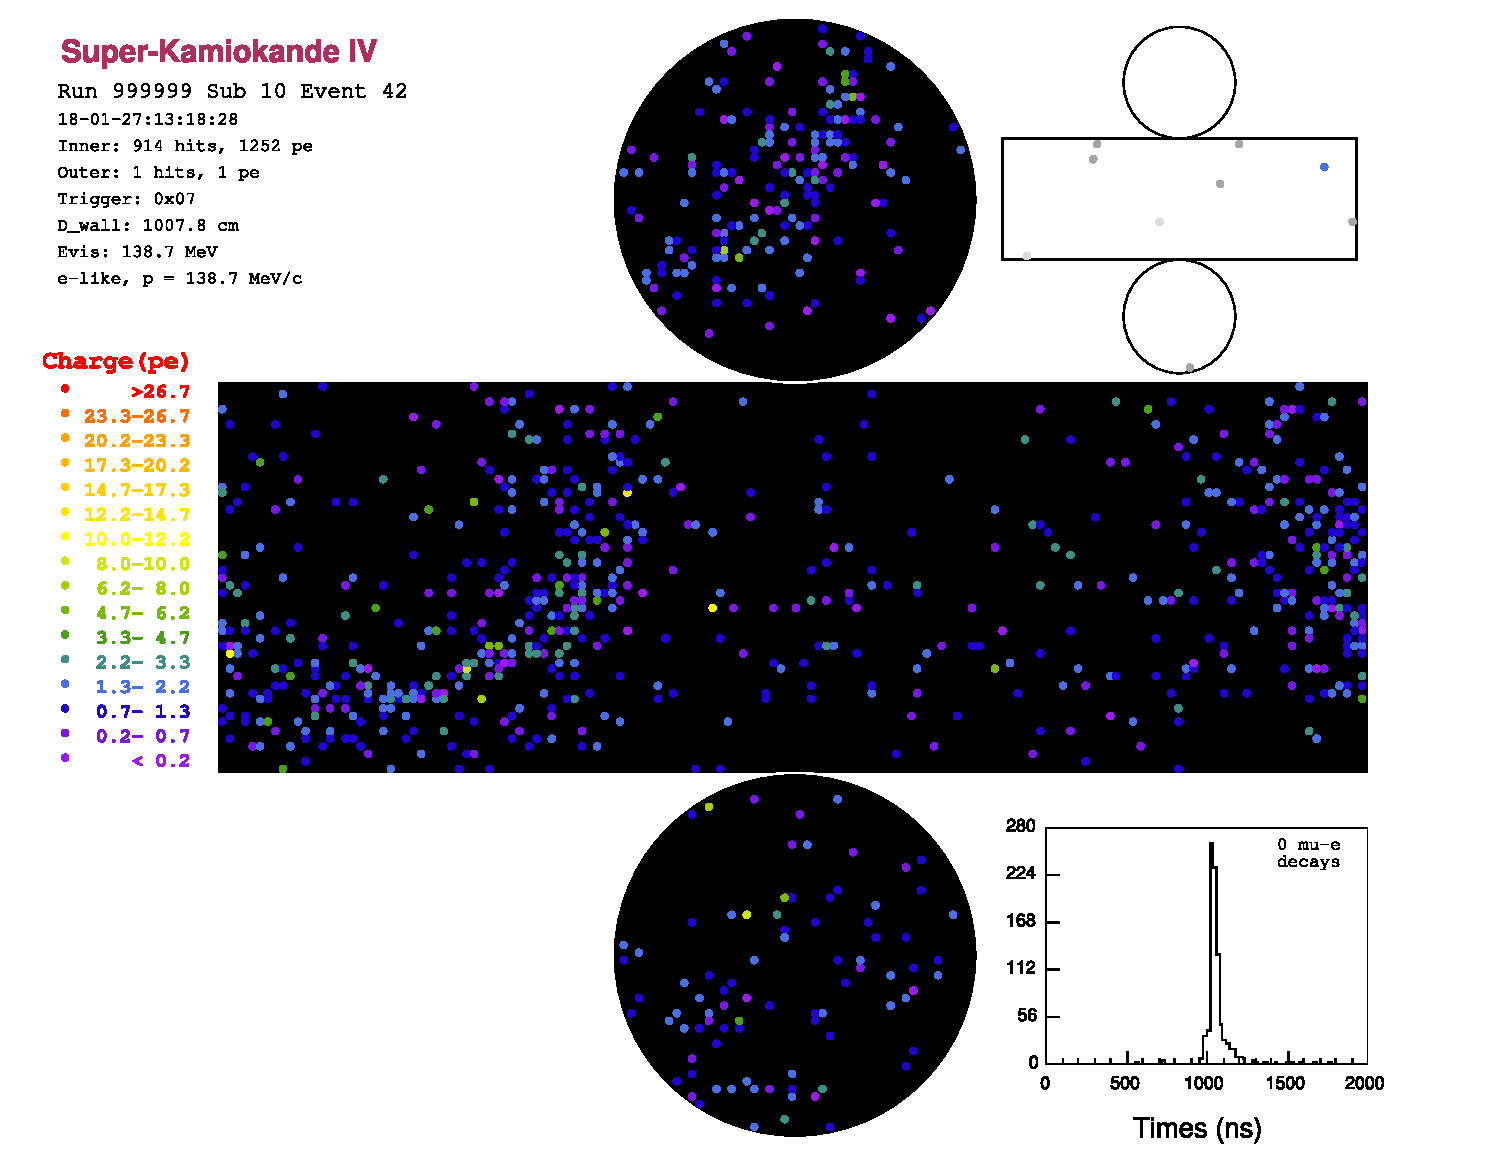
\includegraphics[width=0.45\textwidth]{Electron.pdf}
	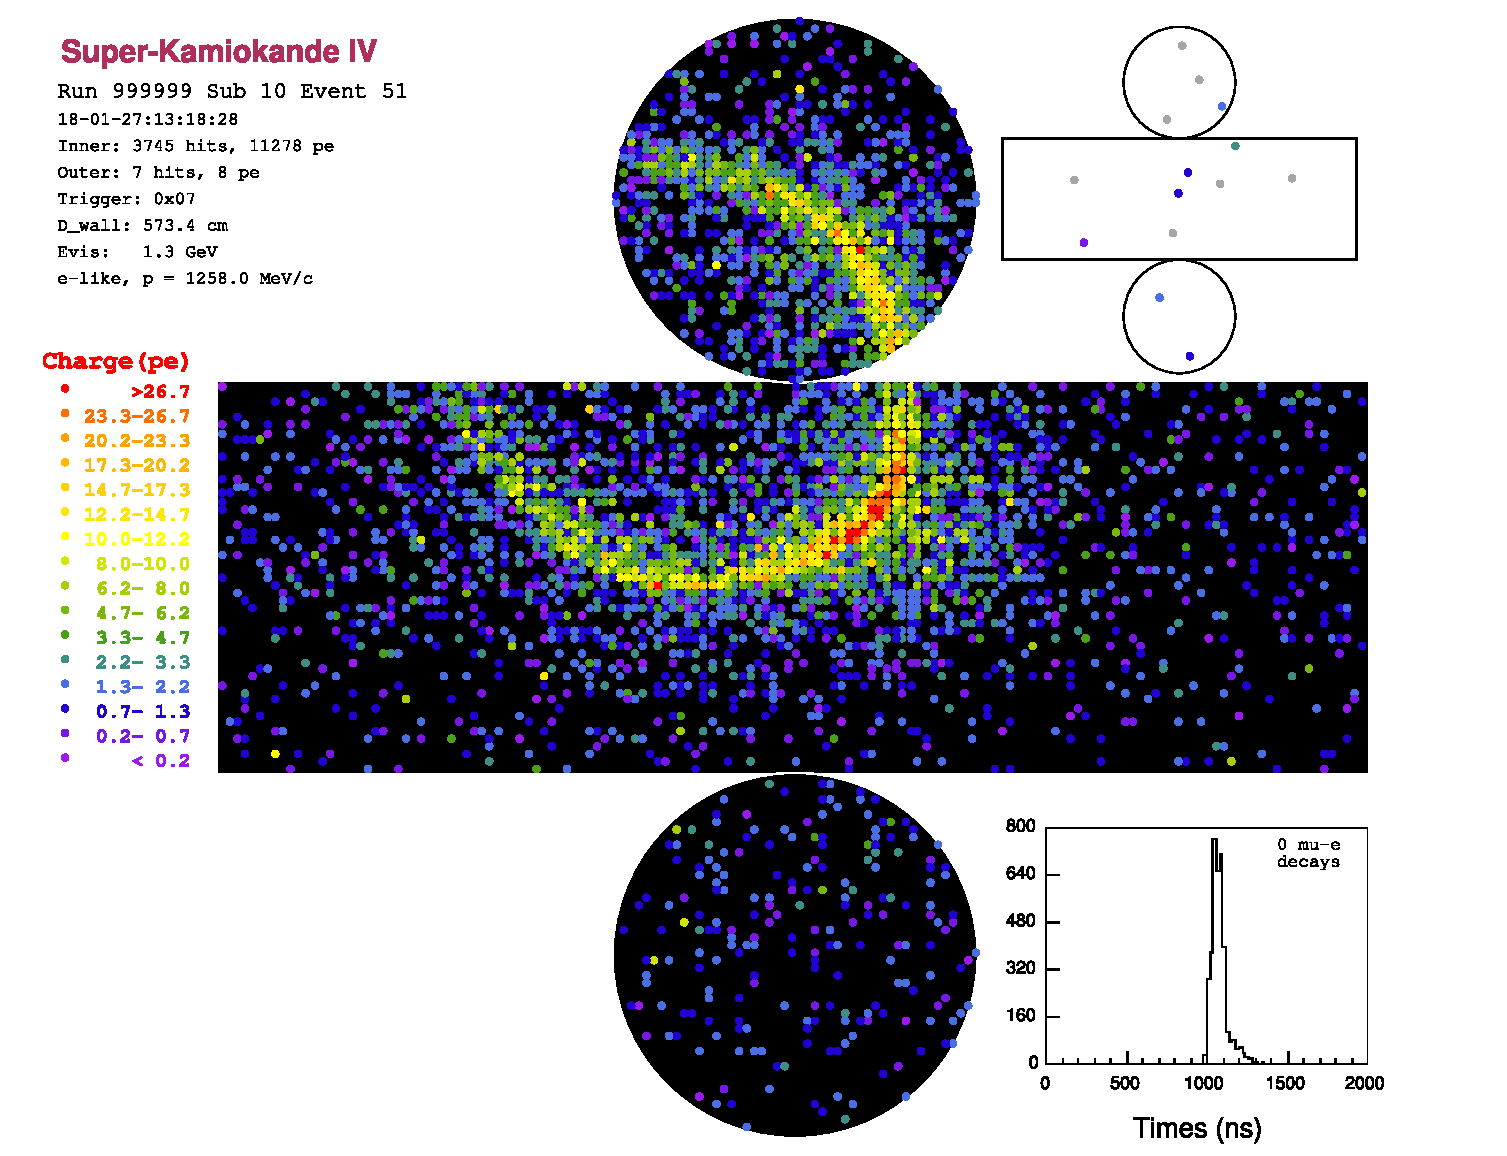
\includegraphics[width=0.45\textwidth]{Muon.pdf}
	\caption{Fully-contained events in the fiducial volume of Super-Kamiokande.}
	\label{fig:sk_events}
\end{figure}

The Super-Kamiokande experiment (SK) is a water Cherenkov detector, %
located in the Kamioka mine, under Mt.\ Ikeno in the Gifu prefecture, Japan.
The rock overburden of $\sim\np{1000}$\,m (\np{2700}\,m.w.e.), shields very efficiently the experiment %
and only cosmic-rays with energies above 1.3\,TeV can reach the detector: %
the muon flux at SK is about \np{6e-8}\,cm\tapi{-2}s\tapi{-1}sr\tapi{-1}, which translates to a rate of 2\,Hz.
The detector consists of a cylindrical stainless steel tank, with a height of 41.4\,m and a diameter of 39.3\,m, %
and it is filled with 50\,kt of ultra pure water ($18$\,M$\Omega$).
The water region is separated into two concentric cylindrical regions, %
called the inner detector (ID, 33.8\,m in diameter) and the outer detector (OD), the latter working as passive and active veto.
The two regions are separated a 55\,cm insensitive region containing the support structure for the PMTs and their cables.
The ID is instrumented with \np{11129} 20'' Hamamatsu R3600 PMTs, facing towards the inside of the tank.
Since the 2001 implosion accident, the photocathode of the PMTs are protected by UV--transparent acrylic domes %
and the side with fiber-reinforced plastic.
The photo coverage of the inner surface is around 40\,\%; the remaining surface not occupied by a PMT is %
lined with black sheet to reduce light reflection.
The main goal of the OD is to tag events originating or finishing outside the ID.
It is instrumented with \np{1885} 8'' Hamamatsu R1408 PMTs which are optically coupled to wavelength shifting plates %
to increase light collectionto increases light collection.
Sheets of white tyvek maximise the propagation of photons inside the ID and helps the reconstruction of corner-clipping events.

The refractive index of water in the visible and ultraviolet region is $n \geq 1.33$, %
and so a charged particle can emit Cherenkov radiation if it is travelling %
with speed $\beta \gtrsim 0.75$.
This converts to an energy threshold of \np{0.78}\,MeV for electrons, \np{160.26}\,MeV for muons, %
\np{211.69}\,MeV for pions, and \np{1423.13}\,MeV for protons, which are the particles usually detected in SK.
The Cherenkov photons, thanks to the high-purity water, reach the walls of the tank where they %
are collected by the PMTs, forming ring patterns.
From the time and charge deposited on the PMTs, the event reconstruction algorithm extracts information of the event %
such as vertex, direction, and energy.
%High energy events, for which $\beta \simeq 1$, generates Cherenkov rings with the same conic angle, %
%which is $\theta \simeq 41^\circ$ in water. 
The same algorithm performs particle identification by looking at the topology and the multiplicity of the ring patterns: %
for example, an electron travelling in the water is more likely to be scattered compared to a muon, %
that on the other hand will follow a more straight path, and as a consquence %
the electron-induced ring is less defined and fuzzier than the muon-induced one.
This can be appreciated on the reconstructed events of \reffig{fig:sk_events}.
Pions usually interact hadronically nuclei with oxygen nuclei, and therefore they have shorter %
and the Cherenkov rings are also less defined than a muon ones.
Muon and pion events can be accompanied by secondary rings from the electrons produced in their decays.
Energetic gamma rays can also be detected, as for instance the ones from $\pi^0$ decays, %
through rings of electrons accelerated by compton scattering.


As part of the strategies to tackle backgrounds, typically only events originating at the centre %
of the ID are considered to be valid.
The materials of the walls of the tank, and particulary the glass of PMTs, contains radioactive material, %
such as isotopes of thorium, uranium and potassium.
These impurities can mimic a signal event in the MeV energy region, crucial for solar neutrino studies.
The selection algorithm simply discards any reconstructed event the vertex of which is less than 200\,cm away from the ID walls.
This criteria defines a fiducial volume (FV), which is around 22.5\,kt in water mass.
The water used to fill the tank may also contain impurities, among which radon, that cause background events.
The water in the tank is continuously filtered at a flow rate of 60\,t/hour by a water purification system.
An air purification system pumps radon-free air into the SK area inside the mine.
This prevents radon in the air to dissolve in the purified water.
Radon contamination is usually less than 3\,mBq/m\tapi{3}, compared to unpurifies air that can peak %
at about 1200\,Bq/m\tapi{3}.
Thanks to these precautions the current energy threshold for SK is \np{3.5}\,MeV.
The main oscillation analyses of SK consider only events originating inside the FV and fully-contained, %
i.e.\ that do not propagate in the OD, as this is signature is given mostly by neutrino interactions.

\section{Neutrons in Super-Kamiokande}
\label{sec:sk_neutron}


Super-Kamiokande and other large scale water Cherenkov detectors have provided %
many evidences in the experimental understanding of neutrinos, %
be it originated in solar, atmospheric, or accelerator facilities.
Despite the large exposure of the experiment, some studies are still curbed by statistical uncertainty %
and would benefit from simply collecting more data.
Other searches, instead, suffer from irreducible background events, as for example the detection of Relic Supernova Neutrinos (SNR), %
%One of the main motivation to detect neutrons is to be able to detect relic supernova neutrinos, %
also know as Diffuse Supernova Neutrino Background (DSNB), an incoherent background spectrum %
produced from all previous core-collapse supernova explosions in the Universe (see \refsec{sec:nu_sun_sn}).
The observation of SNR would be of great importance for improving our knowledge on the population of core-collapse SN %
and the rate of star formation.
The predictions provide with several limits but although SK has the best world limit, no SRN has been detected yet.
The average energies of these neutrinos are around a few tens of MeV, at which the largest cross section %
corresponds to inverse beta decay (IBD, see \refsec{sec:ibd}).
%which is two orders of magnitude larger than $\nu_e$ elastic scattering.
This measurement is afflicted at low energies by invisible muon decay%
---muons below Cherenkov threshold that decay into electrons---and at high energies, %
between $14\,\text{MeV} < E_\nu < 30\,\text{MeV}$, by atmospheric neutrinos.
The energy threshold is also limited by muon-induced spallation events and solar neutrinos, that could be successfully %
rejected with neutron tagging.
If we could detect neutrons efficiently, these backgrounds could be reduced significantly and thus, %
making the detection of the DSNB possible for the first time.

Searches of galactic supernova burst could also avail of an improved background suppression.
SK will be exposed to a huge number of neutrino events if a core-collapse supernova occurs inside our galaxy, %
providing not only an early warning system for other observatories (see \refsec{sec:nu_sun_ns}), %
but also information about the neutrino spectrum, time profile, and information about early stages of the core-collapse process, %
such as pre-supernova neutrinos from the silicon burning phase~\cite{1908.07551}.
The majority of neutrinos emitted are actually antineutrinos in the energies where IBD cross-section dominates.
Detecting the neutron in the final state can be fundamental in distinguishing whether the incoming particle is %
a neutrino or an antineutrino.

Improved neutron tagging is also helpful to understand atmospheric and accelerator neutrino interactions and final states, %
thanks to the capability of separating neutrino and antineutrino interactions.
Finally, the background in proton decay searches can be reduced, since it requires no neutrons to appear in the final state.

%Among these background sources, flasher events\footnote{A flasher event refers to the phenomenon %
%	in which a PMT mis-fires and many repetitive internal discharges are triggered also on nearby PMTs.
%	Flasher events tend to have a broader hit timing distribution than neutrino events.} %

\subsection{Neutron tagging}

Since neutrons are chargeless, they cannot interact with matter by means of the Coulomb force, %
which dominates the energy loss mechanisms for charged particles, described by the Bethe formula.
Neutrons can interact with nuclei in various way, depending on the energy:
\begin{itemize}
	\item elastic and inelastic scattering;
	\item transmutation;
	\item neutron activation;
	\item spallation reaction;
	\item neutron-induced fission;
\end{itemize}

As a result of the interaction, the neutron may either be absorbed, or change its energy and direction significantly.
In this way the average energy of a neutron beam can be completely or partly reduced up to thermal energies, %
close to \np{0.025}~eV.
In this range of energy, the neutron presents a different and often much larger effective neutron absorption %
cross-section for a given nuclide, compared to, for instance, fast neutrons, hence \emph{thermalisation} can %
result in a \emph{neutron activation} process.
This occurs when atomic nuclei capture free thermal neutrons, creating heavier nuclei, often in an excited state.
The excited nucles decays almost instantaneously emitting usually gamma rays.

The neutron energy distribution is adopted to the Maxwellian distribution known for thermal motion.
The time required by the thermalisation of neutrons follows an exponential, and the time constant is largely %
studied, [ref needed], amongst all the thermalisation in water.
It was found that neutron thermalisation in water has a time constant of 5$\mu$s [fujino, sumita, shiba].
Neutrons can be captured by either the hydrogen or the oxygen.
Free neutron will capture on a hydrogen nucleus, releasing a 2.2 MeV gamma.
In SK, for instance, this gamma results in about seven photo-electrons, and thus only detectable with $\simeq$20\,\% %
efficiency.
\begin{figure}
	\centering
	\begin{fmffile}{ibd}
		\begin{fmfgraph*}(100,75)
			\fmfset{arrow_len}{3mm}
			\fmfleft{i2,i1}
			\fmfright{o2,o1}
			\fmf{fermion}{v1,i1}
			\fmf{fermion}{o1,v1}
			\fmf{boson, l.d = 1pt, l.s=left, label=$\!\!W^-\!\!$}{v1,v2}
			\fmf{fermion}{i2,v2}
			\fmf{fermion}{v2,o2}
			\fmfv{l=$\cj{\nu}_e$, l.d=2pt}{i1}
			\fmfv{l=$e^+$, l.d=2pt}{o1}
			\fmfv{l=$p$, l.d=3pt}{i2}
			\fmfv{l=$n$, l.d=3pt}{o2}
			\fmffreeze
			\begin{fmfgroup}
				\fmfset{arrow_len}{1.8mm}
				\fmfpen{0.6thick}
				\fmfi{fermion}{vpath (__i2,__v2) shifted (thick*(0,-2))}
				\fmfi{fermion}{vpath (__i2,__v2) shifted (thick*(0,-4))}
				\fmfi{fermion}{vpath (__v2,__o2) shifted (thick*(0,-2))}
				\fmfi{fermion}{vpath (__v2,__o2) shifted (thick*(0,-4))}
			\end{fmfgroup}
		\end{fmfgraph*}
	\end{fmffile}
	\smallskip
	\caption{Inverse beta decay.}
\end{figure}

\subsection{Neutron calibration}

%https://arxiv.org/pdf/0811.0735.pdf
%https://www.sno.phy.queensu.ca/sno/papers/labranche_phd.pdf
%https://www.sno.phy.queensu.ca/sno/papers/lyon_phd.pdf

To measure neutron tagging efficiency, an americium-beryllium (Am-Be) source is placed inside
a bismuth germanite (BGO) crystal scintillator and the whole device is usually deployed %
at the centre of the water Cherenkov detector.
The americium-241 goes through $\alpha$ decay with a half-life of 432.6\,y. [100\% ?]
The $\alpha$ particle is captured by the \tapi{9}Be nuclei to become \tapi{12}C\tapi{*} with the emission of a neutron.
The carbon de-excites to the ground state with sometimes the emission of a 4.43\,MeV photon.
The gamma ray is promptly captured by the BGO crystal, and the scintillation light triggers the detector.
The neutron thermalises in the water with an average time of roughly 200\,\textmu s, %
before begin captured on a hydrogen nucleus with the release of a 2.2\,MeV photon.
Neutron tagging efficiency on hydrogen in SK was measured to be $(19.0\pm0.2)$\,\%, %
using a unbinned maximum likelihood fitting~\cite{}.
Neutrons released by beryllium have an energy ranging from 2-10 MeV, %
much less than the average neutron energy following atmospheric neutrino interactions.
Thus, we can make the assumption that the location of the Am-Be apparatus is roughly the same %
as the neutron capture vertex.


Another possible source for neutron calibration is californium-252, which %
undergoes $\alpha$-emissions (96.91\%) and spontaneous fission (SF) (3.09\%).
With a half-life of 2.645\,y, a \tapi{252}Cf source has a higher activity compared to an Am-Be source %
with the same number of nucleons.
Furthermore, the SF process emits an average of 3.75 neutrons per fission and an average of 10.3 photons %
having a total energy of 8.2\,Mev.
As for the case of Am-Be, the photons can be collected by a scintillating material to tag the %
emission of neutrons.
After this trigger signal, multiple neutron captures on hydrogen are expected, %
separated by short intervals in time.
The yield of multiple neutrons is another advantage of \tapi{252}Cf that %
the SNO collaboration exploited to develop a method, called \emph{Time Series Analysis} method that uses %
multiplicity and time intervals between the detected events %
to find the neutron detection efficiency, the neutron mean life inside the detector, %
and activity from non-fission events.
The fast-neutron and photon energy spectra are shown in \ref{fig:spectra}: %
the neutrons are emitted with a most-probable energy of 0.7\,MeV and an average energy of 2.1\,MeV.

\begin{figure}
	\begin{minipage}[t]{0.45\textwidth}
		\centering
		\resizebox{\textwidth}{!}{% GNUPLOT: LaTeX picture with Postscript
\begingroup
  \makeatletter
  \providecommand\color[2][]{%
    \GenericError{(gnuplot) \space\space\space\@spaces}{%
      Package color not loaded in conjunction with
      terminal option `colourtext'%
    }{See the gnuplot documentation for explanation.%
    }{Either use 'blacktext' in gnuplot or load the package
      color.sty in LaTeX.}%
    \renewcommand\color[2][]{}%
  }%
  \providecommand\includegraphics[2][]{%
    \GenericError{(gnuplot) \space\space\space\@spaces}{%
      Package graphicx or graphics not loaded%
    }{See the gnuplot documentation for explanation.%
    }{The gnuplot epslatex terminal needs graphicx.sty or graphics.sty.}%
    \renewcommand\includegraphics[2][]{}%
  }%
  \providecommand\rotatebox[2]{#2}%
  \@ifundefined{ifGPcolor}{%
    \newif\ifGPcolor
    \GPcolortrue
  }{}%
  \@ifundefined{ifGPblacktext}{%
    \newif\ifGPblacktext
    \GPblacktexttrue
  }{}%
  % define a \g@addto@macro without @ in the name:
  \let\gplgaddtomacro\g@addto@macro
  % define empty templates for all commands taking text:
  \gdef\gplbacktext{}%
  \gdef\gplfronttext{}%
  \makeatother
  \ifGPblacktext
    % no textcolor at all
    \def\colorrgb#1{}%
    \def\colorgray#1{}%
  \else
    % gray or color?
    \ifGPcolor
      \def\colorrgb#1{\color[rgb]{#1}}%
      \def\colorgray#1{\color[gray]{#1}}%
      \expandafter\def\csname LTw\endcsname{\color{white}}%
      \expandafter\def\csname LTb\endcsname{\color{black}}%
      \expandafter\def\csname LTa\endcsname{\color{black}}%
      \expandafter\def\csname LT0\endcsname{\color[rgb]{1,0,0}}%
      \expandafter\def\csname LT1\endcsname{\color[rgb]{0,1,0}}%
      \expandafter\def\csname LT2\endcsname{\color[rgb]{0,0,1}}%
      \expandafter\def\csname LT3\endcsname{\color[rgb]{1,0,1}}%
      \expandafter\def\csname LT4\endcsname{\color[rgb]{0,1,1}}%
      \expandafter\def\csname LT5\endcsname{\color[rgb]{1,1,0}}%
      \expandafter\def\csname LT6\endcsname{\color[rgb]{0,0,0}}%
      \expandafter\def\csname LT7\endcsname{\color[rgb]{1,0.3,0}}%
      \expandafter\def\csname LT8\endcsname{\color[rgb]{0.5,0.5,0.5}}%
    \else
      % gray
      \def\colorrgb#1{\color{black}}%
      \def\colorgray#1{\color[gray]{#1}}%
      \expandafter\def\csname LTw\endcsname{\color{white}}%
      \expandafter\def\csname LTb\endcsname{\color{black}}%
      \expandafter\def\csname LTa\endcsname{\color{black}}%
      \expandafter\def\csname LT0\endcsname{\color{black}}%
      \expandafter\def\csname LT1\endcsname{\color{black}}%
      \expandafter\def\csname LT2\endcsname{\color{black}}%
      \expandafter\def\csname LT3\endcsname{\color{black}}%
      \expandafter\def\csname LT4\endcsname{\color{black}}%
      \expandafter\def\csname LT5\endcsname{\color{black}}%
      \expandafter\def\csname LT6\endcsname{\color{black}}%
      \expandafter\def\csname LT7\endcsname{\color{black}}%
      \expandafter\def\csname LT8\endcsname{\color{black}}%
    \fi
  \fi
    \setlength{\unitlength}{0.0500bp}%
    \ifx\gptboxheight\undefined%
      \newlength{\gptboxheight}%
      \newlength{\gptboxwidth}%
      \newsavebox{\gptboxtext}%
    \fi%
    \setlength{\fboxrule}{0.5pt}%
    \setlength{\fboxsep}{1pt}%
\begin{picture}(7200.00,5040.00)%
    \gplgaddtomacro\gplbacktext{%
      \csname LTb\endcsname%%
      \put(946,704){\makebox(0,0)[r]{\strut{}$10^{-5}$}}%
      \put(946,1527){\makebox(0,0)[r]{\strut{}$10^{-4}$}}%
      \put(946,2350){\makebox(0,0)[r]{\strut{}$10^{-3}$}}%
      \put(946,3173){\makebox(0,0)[r]{\strut{}$10^{-2}$}}%
      \put(946,3996){\makebox(0,0)[r]{\strut{}$10^{-1}$}}%
      \put(946,4819){\makebox(0,0)[r]{\strut{}$10^{0}$}}%
      \put(1078,484){\makebox(0,0){\strut{}$0$}}%
      \put(1794,484){\makebox(0,0){\strut{}$1$}}%
      \put(2509,484){\makebox(0,0){\strut{}$2$}}%
      \put(3225,484){\makebox(0,0){\strut{}$3$}}%
      \put(3941,484){\makebox(0,0){\strut{}$4$}}%
      \put(4656,484){\makebox(0,0){\strut{}$5$}}%
      \put(5372,484){\makebox(0,0){\strut{}$6$}}%
      \put(6087,484){\makebox(0,0){\strut{}$7$}}%
      \put(6803,484){\makebox(0,0){\strut{}$8$}}%
    }%
    \gplgaddtomacro\gplfronttext{%
      \csname LTb\endcsname%%
      \put(198,2761){\rotatebox{-270}{\makebox(0,0){\strut{}Distribution}}}%
      \put(3940,154){\makebox(0,0){\strut{}Energy (MeV)}}%
      \csname LTb\endcsname%%
      \put(6212,4624){\makebox(0,0)[r]{\strut{}$\gamma$}}%
      \csname LTb\endcsname%%
      \put(6212,4360){\makebox(0,0)[r]{\strut{}$n$}}%
    }%
    \gplbacktext
    \put(0,0){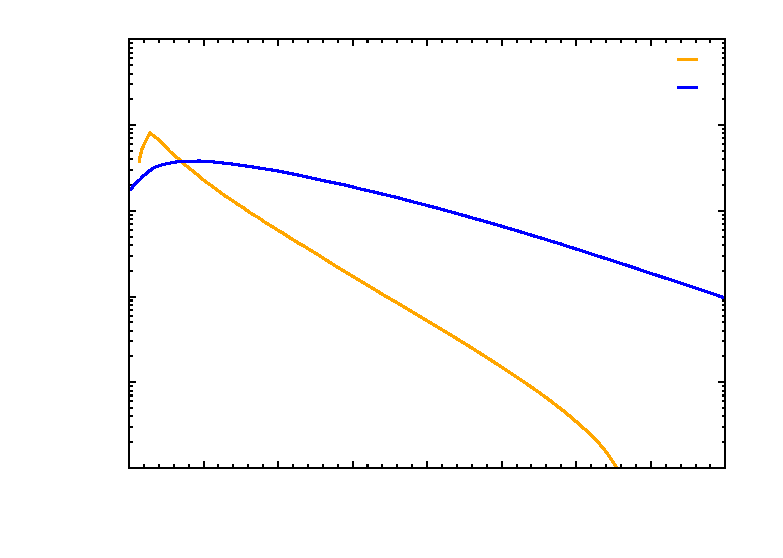
\includegraphics{spectrum}}%
    \gplfronttext
  \end{picture}%
\endgroup
}
		\caption{Normalised energy distribution of neutron and photons emitted %
			by SF events of a \tapi{252}Cf source~\cite{PhysRev.104.699, PhysRev.108.411}.}
		\label{fig:spectra}
	\end{minipage}
	\hfill
	\begin{minipage}[t]{0.56\textwidth}
		\centering
		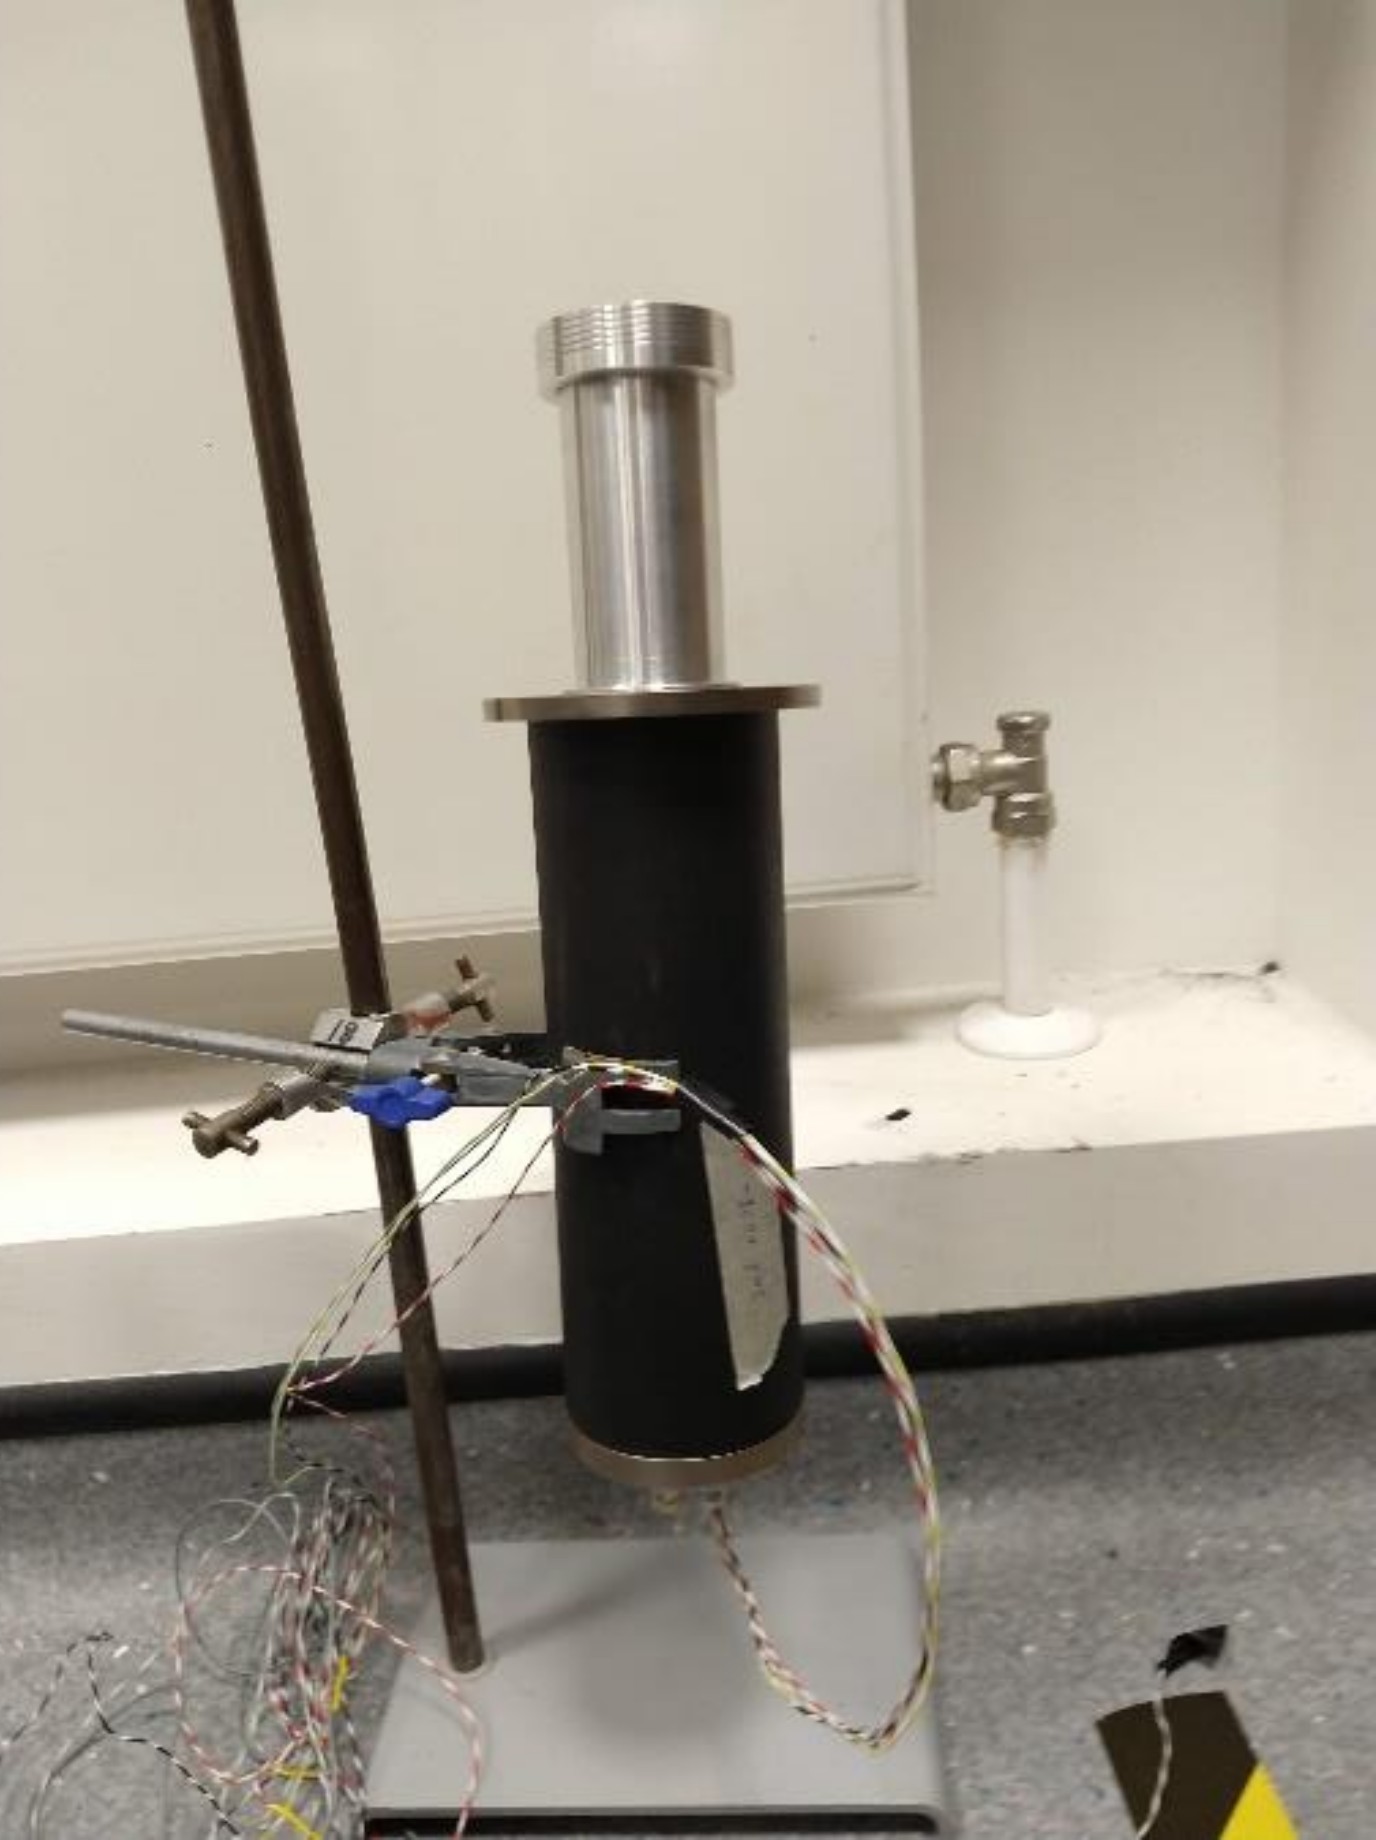
\includegraphics[width=0.4\linewidth]{device.png}
		\raisebox{2.5em}{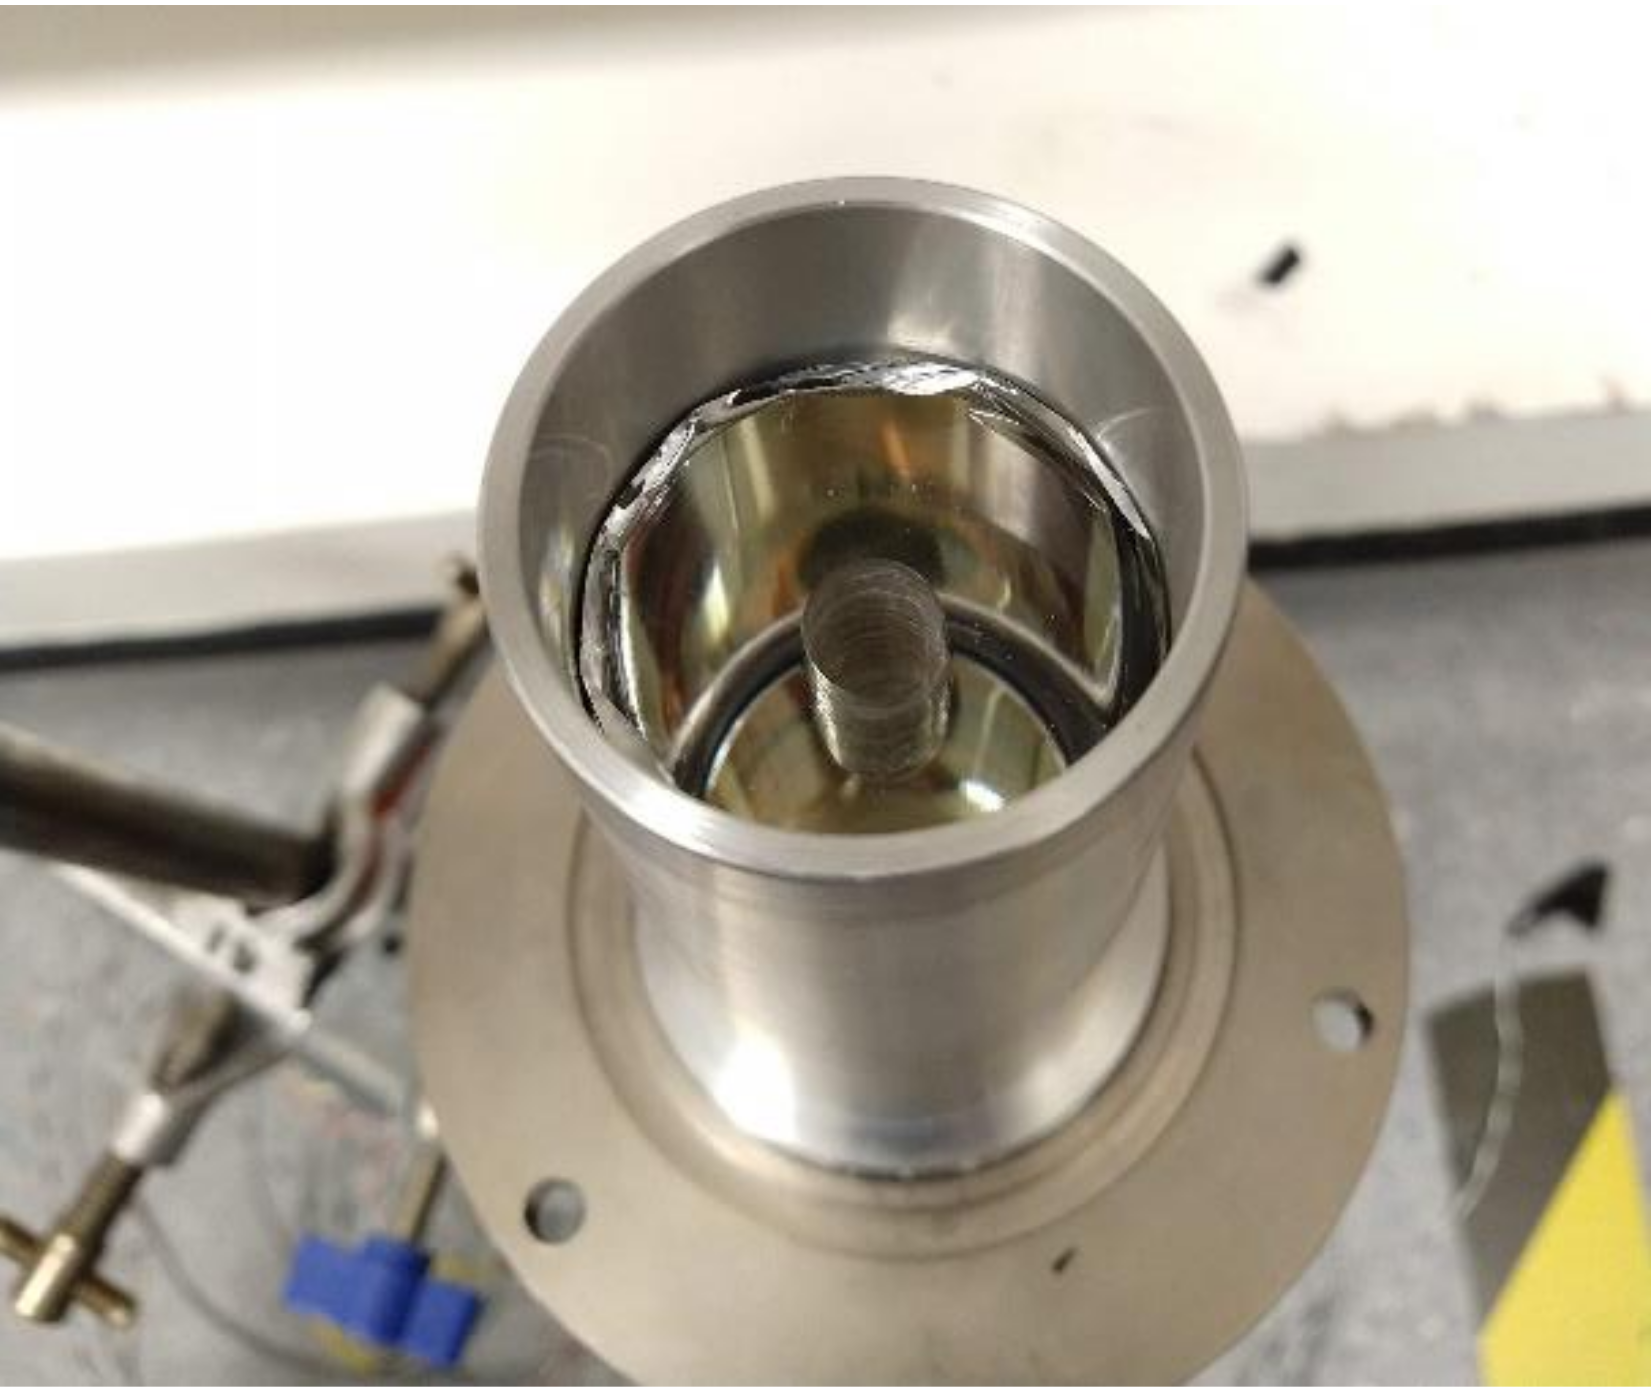
\includegraphics[width=0.4\linewidth]{device_in.png}}
		\captionof{figure}{Setup used to test the californium source.}
		\label{fig:setup}
	\end{minipage}
\end{figure}


A \tapi{252}Cf source was purchased by QMUL with an activity of 4.3\,kBq, measured on the 28\tapi{th} of July, 2017.
The californium is encapsulated in a double hull stainless steel cylinder, 9.5\,mm in diameter and 37.5\,mm high.
The source is tested in a simple calibration device (see Fig.~\ref{fig:setup}), which consists of a cylindrical plastic scintillator %
(EJ-200), coated with mylar to contain optical photons, and optically coupled to a ET Enterprise 9902B series~PMT.
A hole, coaxial to the plastic cylinder, allows to place the source in the middle of the scintillator.
The cylinder is 3\,in in length and 1.5\,in in diameter.
With this setup, the rate of photons emitted by the \tapi{252}Cf source can be measured; %
we used a Struck SIS3316 14-bit VME digitiser to count the number of photon triggers from the PMT and %
a daisy-chain of NIM amplifier, threshold, and discriminator is used before the digitiser to optimise the signal.
Without the source inside the scintillator, an event rate of 1.633\,Hz was measured, whereas with the source inside %
the rate increases to 41.395\,Hz.
The distributions of the PMT peaks collected by the digitiser are shown in Fig.~\ref{fig:source}.
A predicted activity of 3.1\,kBq is expected on the day when the measurement was %
taken---446 days after the activity measurement---which translates to a SF rate of 96.46\,Hz.
The SF tagging efficiency with this setup is therefore around~41\,\%.

\begin{figure}
	\begin{minipage}[t]{0.48\textwidth}
		\centering
		\resizebox{\textwidth}{!}{% GNUPLOT: LaTeX picture with Postscript
\begingroup
  \makeatletter
  \providecommand\color[2][]{%
    \GenericError{(gnuplot) \space\space\space\@spaces}{%
      Package color not loaded in conjunction with
      terminal option `colourtext'%
    }{See the gnuplot documentation for explanation.%
    }{Either use 'blacktext' in gnuplot or load the package
      color.sty in LaTeX.}%
    \renewcommand\color[2][]{}%
  }%
  \providecommand\includegraphics[2][]{%
    \GenericError{(gnuplot) \space\space\space\@spaces}{%
      Package graphicx or graphics not loaded%
    }{See the gnuplot documentation for explanation.%
    }{The gnuplot epslatex terminal needs graphicx.sty or graphics.sty.}%
    \renewcommand\includegraphics[2][]{}%
  }%
  \providecommand\rotatebox[2]{#2}%
  \@ifundefined{ifGPcolor}{%
    \newif\ifGPcolor
    \GPcolortrue
  }{}%
  \@ifundefined{ifGPblacktext}{%
    \newif\ifGPblacktext
    \GPblacktexttrue
  }{}%
  % define a \g@addto@macro without @ in the name:
  \let\gplgaddtomacro\g@addto@macro
  % define empty templates for all commands taking text:
  \gdef\gplbacktext{}%
  \gdef\gplfronttext{}%
  \makeatother
  \ifGPblacktext
    % no textcolor at all
    \def\colorrgb#1{}%
    \def\colorgray#1{}%
  \else
    % gray or color?
    \ifGPcolor
      \def\colorrgb#1{\color[rgb]{#1}}%
      \def\colorgray#1{\color[gray]{#1}}%
      \expandafter\def\csname LTw\endcsname{\color{white}}%
      \expandafter\def\csname LTb\endcsname{\color{black}}%
      \expandafter\def\csname LTa\endcsname{\color{black}}%
      \expandafter\def\csname LT0\endcsname{\color[rgb]{1,0,0}}%
      \expandafter\def\csname LT1\endcsname{\color[rgb]{0,1,0}}%
      \expandafter\def\csname LT2\endcsname{\color[rgb]{0,0,1}}%
      \expandafter\def\csname LT3\endcsname{\color[rgb]{1,0,1}}%
      \expandafter\def\csname LT4\endcsname{\color[rgb]{0,1,1}}%
      \expandafter\def\csname LT5\endcsname{\color[rgb]{1,1,0}}%
      \expandafter\def\csname LT6\endcsname{\color[rgb]{0,0,0}}%
      \expandafter\def\csname LT7\endcsname{\color[rgb]{1,0.3,0}}%
      \expandafter\def\csname LT8\endcsname{\color[rgb]{0.5,0.5,0.5}}%
    \else
      % gray
      \def\colorrgb#1{\color{black}}%
      \def\colorgray#1{\color[gray]{#1}}%
      \expandafter\def\csname LTw\endcsname{\color{white}}%
      \expandafter\def\csname LTb\endcsname{\color{black}}%
      \expandafter\def\csname LTa\endcsname{\color{black}}%
      \expandafter\def\csname LT0\endcsname{\color{black}}%
      \expandafter\def\csname LT1\endcsname{\color{black}}%
      \expandafter\def\csname LT2\endcsname{\color{black}}%
      \expandafter\def\csname LT3\endcsname{\color{black}}%
      \expandafter\def\csname LT4\endcsname{\color{black}}%
      \expandafter\def\csname LT5\endcsname{\color{black}}%
      \expandafter\def\csname LT6\endcsname{\color{black}}%
      \expandafter\def\csname LT7\endcsname{\color{black}}%
      \expandafter\def\csname LT8\endcsname{\color{black}}%
    \fi
  \fi
    \setlength{\unitlength}{0.0500bp}%
    \ifx\gptboxheight\undefined%
      \newlength{\gptboxheight}%
      \newlength{\gptboxwidth}%
      \newsavebox{\gptboxtext}%
    \fi%
    \setlength{\fboxrule}{0.5pt}%
    \setlength{\fboxsep}{1pt}%
\begin{picture}(7200.00,5040.00)%
    \gplgaddtomacro\gplbacktext{%
      \csname LTb\endcsname%%
      \put(1078,704){\makebox(0,0)[r]{\strut{}$10^{-3}$}}%
      \put(1078,1733){\makebox(0,0)[r]{\strut{}$10^{-2}$}}%
      \put(1078,2762){\makebox(0,0)[r]{\strut{}$0.1$}}%
      \put(1078,3790){\makebox(0,0)[r]{\strut{}$1$}}%
      \put(1078,4819){\makebox(0,0)[r]{\strut{}$10$}}%
      \put(1210,484){\makebox(0,0){\strut{}$0$}}%
      \put(2142,484){\makebox(0,0){\strut{}$0.1$}}%
      \put(3074,484){\makebox(0,0){\strut{}$0.2$}}%
      \put(4007,484){\makebox(0,0){\strut{}$0.3$}}%
      \put(4939,484){\makebox(0,0){\strut{}$0.4$}}%
      \put(5871,484){\makebox(0,0){\strut{}$0.5$}}%
      \put(6803,484){\makebox(0,0){\strut{}$0.6$}}%
    }%
    \gplgaddtomacro\gplfronttext{%
      \csname LTb\endcsname%%
      \put(298,2761){\rotatebox{-270}{\makebox(0,0){\strut{}Events / s}}}%
      \put(4006,154){\makebox(0,0){\strut{}Peak (V)}}%
      \csname LTb\endcsname%%
      \put(6212,4624){\makebox(0,0)[r]{\strut{}Source in}}%
      \csname LTb\endcsname%%
      \put(6212,4360){\makebox(0,0)[r]{\strut{}Source out}}%
    }%
    \gplbacktext
    \put(0,0){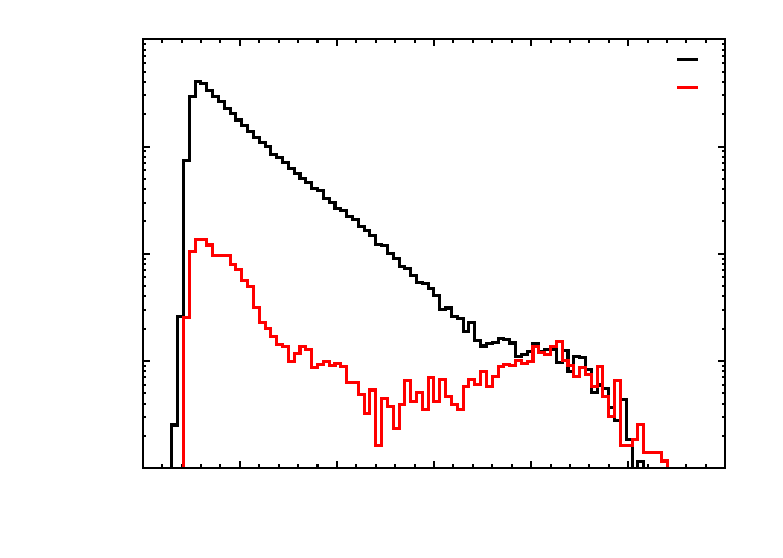
\includegraphics{pics/peaksources}}%
    \gplfronttext
  \end{picture}%
\endgroup
}
		\captionof{figure}{Distribution of PMT peaks measured with source inside (black) and source removed from the scintillator~(red).}
		\label{fig:source}
	\end{minipage}
	\hfill
	\begin{minipage}[t]{0.48\textwidth}
		\centering
		\resizebox{\textwidth}{!}{% GNUPLOT: LaTeX picture with Postscript
\begingroup
  \makeatletter
  \providecommand\color[2][]{%
    \GenericError{(gnuplot) \space\space\space\@spaces}{%
      Package color not loaded in conjunction with
      terminal option `colourtext'%
    }{See the gnuplot documentation for explanation.%
    }{Either use 'blacktext' in gnuplot or load the package
      color.sty in LaTeX.}%
    \renewcommand\color[2][]{}%
  }%
  \providecommand\includegraphics[2][]{%
    \GenericError{(gnuplot) \space\space\space\@spaces}{%
      Package graphicx or graphics not loaded%
    }{See the gnuplot documentation for explanation.%
    }{The gnuplot epslatex terminal needs graphicx.sty or graphics.sty.}%
    \renewcommand\includegraphics[2][]{}%
  }%
  \providecommand\rotatebox[2]{#2}%
  \@ifundefined{ifGPcolor}{%
    \newif\ifGPcolor
    \GPcolortrue
  }{}%
  \@ifundefined{ifGPblacktext}{%
    \newif\ifGPblacktext
    \GPblacktexttrue
  }{}%
  % define a \g@addto@macro without @ in the name:
  \let\gplgaddtomacro\g@addto@macro
  % define empty templates for all commands taking text:
  \gdef\gplbacktext{}%
  \gdef\gplfronttext{}%
  \makeatother
  \ifGPblacktext
    % no textcolor at all
    \def\colorrgb#1{}%
    \def\colorgray#1{}%
  \else
    % gray or color?
    \ifGPcolor
      \def\colorrgb#1{\color[rgb]{#1}}%
      \def\colorgray#1{\color[gray]{#1}}%
      \expandafter\def\csname LTw\endcsname{\color{white}}%
      \expandafter\def\csname LTb\endcsname{\color{black}}%
      \expandafter\def\csname LTa\endcsname{\color{black}}%
      \expandafter\def\csname LT0\endcsname{\color[rgb]{1,0,0}}%
      \expandafter\def\csname LT1\endcsname{\color[rgb]{0,1,0}}%
      \expandafter\def\csname LT2\endcsname{\color[rgb]{0,0,1}}%
      \expandafter\def\csname LT3\endcsname{\color[rgb]{1,0,1}}%
      \expandafter\def\csname LT4\endcsname{\color[rgb]{0,1,1}}%
      \expandafter\def\csname LT5\endcsname{\color[rgb]{1,1,0}}%
      \expandafter\def\csname LT6\endcsname{\color[rgb]{0,0,0}}%
      \expandafter\def\csname LT7\endcsname{\color[rgb]{1,0.3,0}}%
      \expandafter\def\csname LT8\endcsname{\color[rgb]{0.5,0.5,0.5}}%
    \else
      % gray
      \def\colorrgb#1{\color{black}}%
      \def\colorgray#1{\color[gray]{#1}}%
      \expandafter\def\csname LTw\endcsname{\color{white}}%
      \expandafter\def\csname LTb\endcsname{\color{black}}%
      \expandafter\def\csname LTa\endcsname{\color{black}}%
      \expandafter\def\csname LT0\endcsname{\color{black}}%
      \expandafter\def\csname LT1\endcsname{\color{black}}%
      \expandafter\def\csname LT2\endcsname{\color{black}}%
      \expandafter\def\csname LT3\endcsname{\color{black}}%
      \expandafter\def\csname LT4\endcsname{\color{black}}%
      \expandafter\def\csname LT5\endcsname{\color{black}}%
      \expandafter\def\csname LT6\endcsname{\color{black}}%
      \expandafter\def\csname LT7\endcsname{\color{black}}%
      \expandafter\def\csname LT8\endcsname{\color{black}}%
    \fi
  \fi
    \setlength{\unitlength}{0.0500bp}%
    \ifx\gptboxheight\undefined%
      \newlength{\gptboxheight}%
      \newlength{\gptboxwidth}%
      \newsavebox{\gptboxtext}%
    \fi%
    \setlength{\fboxrule}{0.5pt}%
    \setlength{\fboxsep}{1pt}%
\begin{picture}(7200.00,5040.00)%
    \gplgaddtomacro\gplbacktext{%
      \csname LTb\endcsname%%
      \put(946,2142){\makebox(0,0)[r]{\strut{}$0.05$}}%
      \put(946,4200){\makebox(0,0)[r]{\strut{}$0.5$}}%
      \put(946,704){\makebox(0,0)[r]{\strut{}$0.01$}}%
      \put(946,2762){\makebox(0,0)[r]{\strut{}$0.1$}}%
      \put(946,4819){\makebox(0,0)[r]{\strut{}$1$}}%
      \put(1460,484){\makebox(0,0){\strut{}$300$}}%
      \put(2223,484){\makebox(0,0){\strut{}$350$}}%
      \put(2986,484){\makebox(0,0){\strut{}$400$}}%
      \put(3750,484){\makebox(0,0){\strut{}$450$}}%
      \put(4513,484){\makebox(0,0){\strut{}$500$}}%
      \put(5276,484){\makebox(0,0){\strut{}$550$}}%
      \put(6040,484){\makebox(0,0){\strut{}$600$}}%
      \put(6803,484){\makebox(0,0){\strut{}$650$}}%
    }%
    \gplgaddtomacro\gplfronttext{%
      \csname LTb\endcsname%%
      \put(198,2761){\rotatebox{-270}{\makebox(0,0){\strut{}Efficiency}}}%
      \put(3940,154){\makebox(0,0){\strut{}Wavelength (nm)}}%
      \csname LTb\endcsname%%
      \put(6212,4624){\makebox(0,0)[r]{\strut{}PMT}}%
      \csname LTb\endcsname%%
      \put(6212,4360){\makebox(0,0)[r]{\strut{}Scintillator}}%
      \csname LTb\endcsname%%
      \put(6212,4096){\makebox(0,0)[r]{\strut{}Correlation}}%
      \csname LTb\endcsname%%
      \put(6212,3832){\makebox(0,0)[r]{\strut{}MC}}%
    }%
    \gplbacktext
    \put(0,0){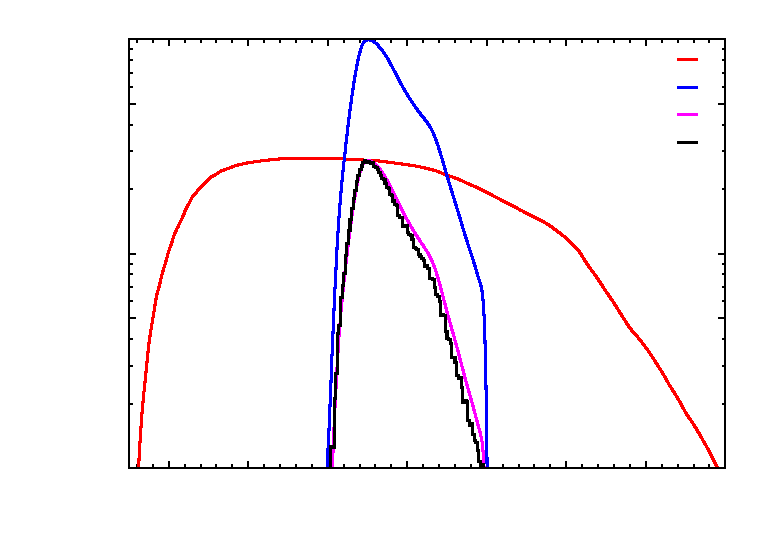
\includegraphics{pics/QE}}%
    \gplfronttext
  \end{picture}%
\endgroup
}
		\captionof{figure}{Plot showing PMT quantum efficiency (red), the scintillator yield (blue), %
			their convolution (magenta) and the distributions of photon collected by the PMT in the GEANT4 simulation of optical photons (black).}
		\label{fig:QE}
	\end{minipage}
\end{figure}

We performed a GEANT4 simulation of the setup, with the aim of optimising the calibration device.
An ideal calibration device would absorb all the photons converting them into visible light without affect the neutrons.
The plot in Fig.~\ref{fig:QE} shows the correct implementation of the scintillator and PMT efficiencies, %
as there is good agreement with the MC distribution and the expected optical photon spectrum.
The scintillating volume is therefore varied in the simulation to study the preformance of the decive.
Bismuth germanate oxide (BGO) crystal and a generic vinyltouluene plastic are studied as scintillating materials.
The size of the scintillator is also varied and shapes of a cube and a cylinder with equal diameter and height are tested.
The simulation keeps track of the energy deposited in the scintillator and the number of neutrons escaping the device.
The result is shown in Fig.~\ref{fig:geant4}.
Unsurprisingly, the BGO crystal performs better than the plastic scintillator, %
with the optimal volume being a cube with 12\,cm sides.
The hydrogen in the plastic thermalises neutrons, which can have an impact on the thermalisation time %
in a water Cherenkov detector.

\begin{figure}
	\centering
	\resizebox{0.9\textwidth}{!}{% GNUPLOT: LaTeX picture with Postscript
\begingroup
  \makeatletter
  \providecommand\color[2][]{%
    \GenericError{(gnuplot) \space\space\space\@spaces}{%
      Package color not loaded in conjunction with
      terminal option `colourtext'%
    }{See the gnuplot documentation for explanation.%
    }{Either use 'blacktext' in gnuplot or load the package
      color.sty in LaTeX.}%
    \renewcommand\color[2][]{}%
  }%
  \providecommand\includegraphics[2][]{%
    \GenericError{(gnuplot) \space\space\space\@spaces}{%
      Package graphicx or graphics not loaded%
    }{See the gnuplot documentation for explanation.%
    }{The gnuplot epslatex terminal needs graphicx.sty or graphics.sty.}%
    \renewcommand\includegraphics[2][]{}%
  }%
  \providecommand\rotatebox[2]{#2}%
  \@ifundefined{ifGPcolor}{%
    \newif\ifGPcolor
    \GPcolortrue
  }{}%
  \@ifundefined{ifGPblacktext}{%
    \newif\ifGPblacktext
    \GPblacktexttrue
  }{}%
  % define a \g@addto@macro without @ in the name:
  \let\gplgaddtomacro\g@addto@macro
  % define empty templates for all commands taking text:
  \gdef\gplbacktext{}%
  \gdef\gplfronttext{}%
  \makeatother
  \ifGPblacktext
    % no textcolor at all
    \def\colorrgb#1{}%
    \def\colorgray#1{}%
  \else
    % gray or color?
    \ifGPcolor
      \def\colorrgb#1{\color[rgb]{#1}}%
      \def\colorgray#1{\color[gray]{#1}}%
      \expandafter\def\csname LTw\endcsname{\color{white}}%
      \expandafter\def\csname LTb\endcsname{\color{black}}%
      \expandafter\def\csname LTa\endcsname{\color{black}}%
      \expandafter\def\csname LT0\endcsname{\color[rgb]{1,0,0}}%
      \expandafter\def\csname LT1\endcsname{\color[rgb]{0,1,0}}%
      \expandafter\def\csname LT2\endcsname{\color[rgb]{0,0,1}}%
      \expandafter\def\csname LT3\endcsname{\color[rgb]{1,0,1}}%
      \expandafter\def\csname LT4\endcsname{\color[rgb]{0,1,1}}%
      \expandafter\def\csname LT5\endcsname{\color[rgb]{1,1,0}}%
      \expandafter\def\csname LT6\endcsname{\color[rgb]{0,0,0}}%
      \expandafter\def\csname LT7\endcsname{\color[rgb]{1,0.3,0}}%
      \expandafter\def\csname LT8\endcsname{\color[rgb]{0.5,0.5,0.5}}%
    \else
      % gray
      \def\colorrgb#1{\color{black}}%
      \def\colorgray#1{\color[gray]{#1}}%
      \expandafter\def\csname LTw\endcsname{\color{white}}%
      \expandafter\def\csname LTb\endcsname{\color{black}}%
      \expandafter\def\csname LTa\endcsname{\color{black}}%
      \expandafter\def\csname LT0\endcsname{\color{black}}%
      \expandafter\def\csname LT1\endcsname{\color{black}}%
      \expandafter\def\csname LT2\endcsname{\color{black}}%
      \expandafter\def\csname LT3\endcsname{\color{black}}%
      \expandafter\def\csname LT4\endcsname{\color{black}}%
      \expandafter\def\csname LT5\endcsname{\color{black}}%
      \expandafter\def\csname LT6\endcsname{\color{black}}%
      \expandafter\def\csname LT7\endcsname{\color{black}}%
      \expandafter\def\csname LT8\endcsname{\color{black}}%
    \fi
  \fi
    \setlength{\unitlength}{0.0500bp}%
    \ifx\gptboxheight\undefined%
      \newlength{\gptboxheight}%
      \newlength{\gptboxwidth}%
      \newsavebox{\gptboxtext}%
    \fi%
    \setlength{\fboxrule}{0.5pt}%
    \setlength{\fboxsep}{1pt}%
\begin{picture}(14400.00,7632.00)%
    \gplgaddtomacro\gplbacktext{%
      \csname LTb\endcsname%%
      \put(444,440){\makebox(0,0)[r]{\strut{}$0$}}%
      \put(444,1789){\makebox(0,0)[r]{\strut{}$0.2$}}%
      \put(444,3138){\makebox(0,0)[r]{\strut{}$0.4$}}%
      \put(444,4486){\makebox(0,0)[r]{\strut{}$0.6$}}%
      \put(444,5835){\makebox(0,0)[r]{\strut{}$0.8$}}%
      \put(444,7184){\makebox(0,0)[r]{\strut{}$1$}}%
      \put(576,220){\makebox(0,0){\strut{}$0$}}%
      \put(2304,220){\makebox(0,0){\strut{}$10$}}%
      \put(4032,220){\makebox(0,0){\strut{}$20$}}%
      \put(5759,220){\makebox(0,0){\strut{}$30$}}%
      \put(4032,3812){\makebox(0,0)[l]{\strut{}BGO scintillator}}%
    }%
    \gplgaddtomacro\gplfronttext{%
      \csname LTb\endcsname%%
      \put(-172,3980){\rotatebox{-270}{\makebox(0,0){\strut{}Percentage (\%)}}}%
      \put(4031,-110){\makebox(0,0){\strut{}Size (cm)}}%
      \csname LTb\endcsname%%
      \put(6896,1273){\makebox(0,0)[r]{\strut{}Gamma aborsbed energy (\%)}}%
      \csname LTb\endcsname%%
      \put(6896,1053){\makebox(0,0)[r]{\strut{}Neutron surviving (\%)}}%
      \csname LTb\endcsname%%
      \put(6896,833){\makebox(0,0)[r]{\strut{}Cube}}%
      \csname LTb\endcsname%%
      \put(6896,613){\makebox(0,0)[r]{\strut{}Cylinder}}%
    }%
    \gplgaddtomacro\gplbacktext{%
      \csname LTb\endcsname%%
      \put(7356,440){\makebox(0,0)[r]{\strut{}}}%
      \put(7356,1789){\makebox(0,0)[r]{\strut{}}}%
      \put(7356,3138){\makebox(0,0)[r]{\strut{}}}%
      \put(7356,4486){\makebox(0,0)[r]{\strut{}}}%
      \put(7356,5835){\makebox(0,0)[r]{\strut{}}}%
      \put(7356,7184){\makebox(0,0)[r]{\strut{}}}%
      \put(14399,220){\makebox(0,0){\strut{}$40$}}%
      \put(7488,220){\makebox(0,0){\strut{}$0$}}%
      \put(9216,220){\makebox(0,0){\strut{}$10$}}%
      \put(10944,220){\makebox(0,0){\strut{}$20$}}%
      \put(12671,220){\makebox(0,0){\strut{}$30$}}%
      \put(10944,3812){\makebox(0,0)[l]{\strut{}Plastic scintillator}}%
    }%
    \gplgaddtomacro\gplfronttext{%
      \csname LTb\endcsname%%
      \put(10943,-110){\makebox(0,0){\strut{}Size (cm)}}%
      \csname LTb\endcsname%%
      \put(13808,7348){\makebox(0,0)[r]{\strut{}Gamma aborsbed energy (\%)}}%
      \csname LTb\endcsname%%
      \put(13808,7128){\makebox(0,0)[r]{\strut{}Neutron surviving (\%)}}%
      \csname LTb\endcsname%%
      \put(13808,6908){\makebox(0,0)[r]{\strut{}Cube}}%
      \csname LTb\endcsname%%
      \put(13808,6688){\makebox(0,0)[r]{\strut{}Cylinder}}%
    }%
    \gplbacktext
    \put(0,0){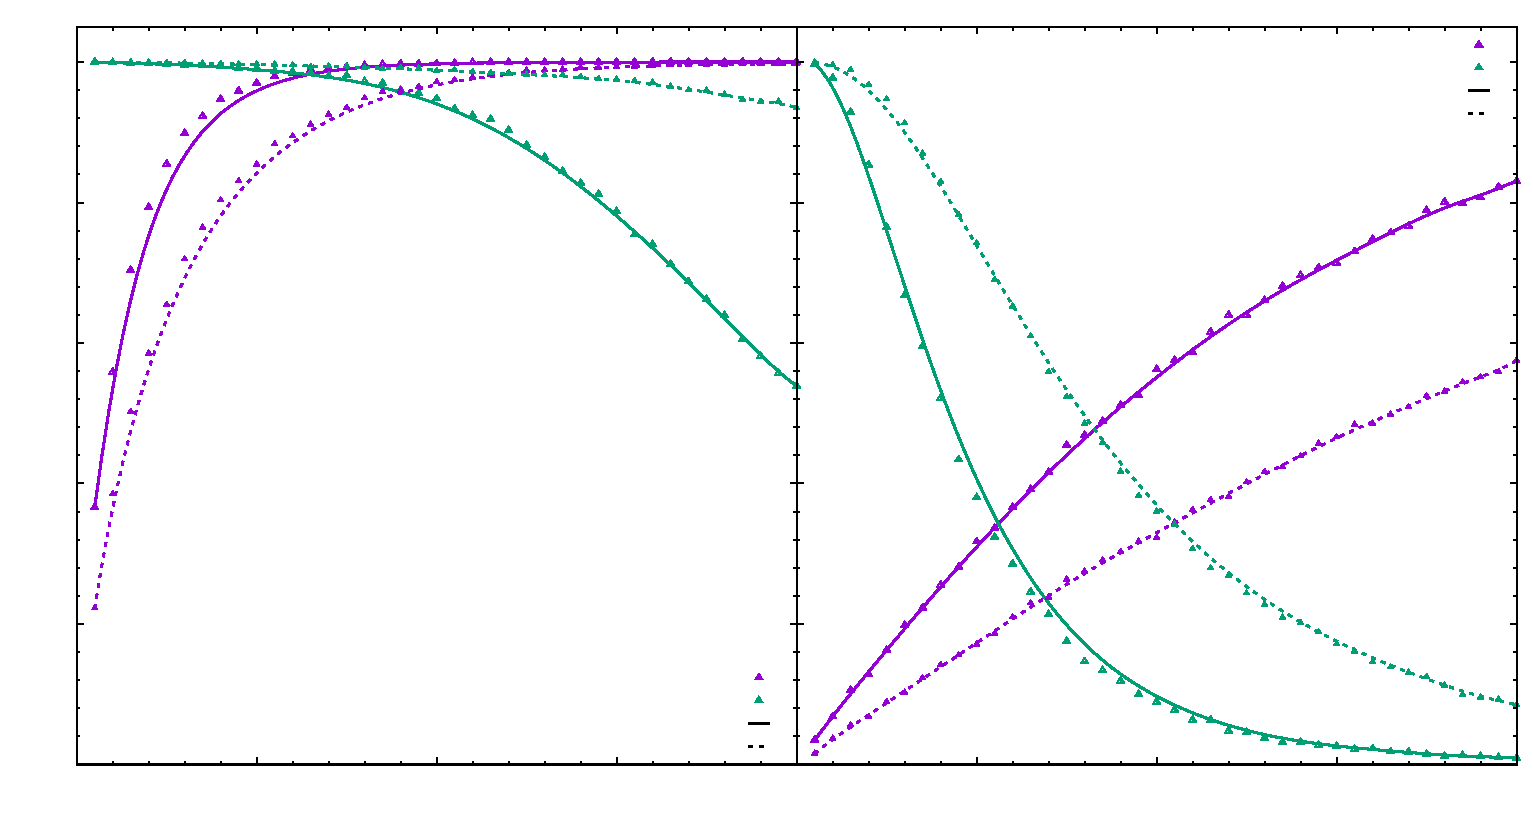
\includegraphics{pics/n_vs_gamma}}%
    \gplfronttext
  \end{picture}%
\endgroup
}
	\caption{Result of the GEANT4 simulation, showing the performance of different scintillators.
		Two shapes are tested: a cube (solid lines) and a cylinder with equal diameter and hie hgt (dashed lines).
		The percentage of energy absorbed by the scintillator (purple) and the percentage of neutrons escaping the %
		scintillators (green) are estimated for every simulation.
		Left: BGO is used as scintillating material. Right: a generic vinyltouluene plastic is used.}
	\label{fig:geant4}
\end{figure}


%To verify neutron tagging efficiency given above, experimental tests were conducted with an Am/Be source embedded in a bismuth germanite (BGO) scintillator. The prompt and delayed event-pair is generated via: α + 9Be →12
%C∗+n; 12C∗ →12 C+γ(prompt); n+p → d+γ(delayed).
%The scintillation light induced by 4.43 MeV deexcitation γ
%serves as the primary event. Note that the reaction to the
%ground state of 12C also exists, where no 4.43 MeV deexcitation γ is emitted. The experimental apparatus was
%deployed at the center of the tank, during which the trigger
%gate to catch 2.2 MeV γ was temporarily enlarged to 800
%μs in order to obtain a complete neutron capture time spectrum. To estimate source related background (e.g. ground
%transition neutron), 10 Hz 800μs random trigger data was
%also taken.
%The final N10 distribution after all cuts applied is shown in
%Fig. 2, where for Am/Be data all backgrounds are subtracted according to random trigger data. Signal efficiencies for
%MC and data are (19.2±0.1)% and (19.0±0.2)%, respectively. Data is in good agreement with MC. Fig. 3 shows
%the distribution of time difference (ΔT) between delayed
%neutron signal and prompt event. The neutron lifetime in
%pure water is measured to be (201.8 ± 4.7)μs using a unbinned maximum likelihood fitting as shown in Fig. 3.
%
%The Am-Be source is embedded in a 5 cm cube of BGO scintillator (see figure 8.27)
%to amplify the light released by the 4.4 MeV γ-ray, such that it will activate the SHE
%trigger in the detector. Upon triggering SHE stores 35µs of data, and then an extended
%AFT trigger is activated to store an additional 800µs, and grant a more complete view
%the neutron capture time spectrum.
%Figure 8.27: Am-Be crystal embedded in a 5 cm cube of BGO scintillator. This is
%held in an acrylic case.
%This configuration was set up in 3 different locations around the tank: the centre (35.3,
%-70.7, 0) cm (Centre), near the side of the barrel (35.3, -1201.9, 0) cm (Y12), and near
%the top of the tank (35.3, -70.7, 1500.0) cm (Z15). Random data was also taken with
%the apparatus in the centre, using a 10Hz trigger, to study the irreducible background
%from the ground-state transition.
%
%
%Neutron tagging is then performed on the remaining Am-Be dataset, and a 2.2 MeV
%γ-ray MC. There are some differences between this study and the atmospheric neutrino study discussed up until now. Neutrons released by Beryllium have an energy
%ranging from 2-10 MeV, much less than the average neutron energy following atmospheric neutrino interactions. Thus, we can make the assumption that the location of
%the Am-Be apparatus is roughly the same as the neutron capture vertex. This raises
%the expected neutron detection efficiency in accordance with figure 8.23. In addition,
%Chapter 8. Neutron Tagging 140
%the PMT after-pulse observed following high energy atmospheric neutrino events (figure 8.5) is not produced to the same extent after Am-Be events, so neutron searching
%is started at 5µs (previously > 18µs) after the primary trigger. The AFT trigger for
%Am-Be is also extended, allowing neutron-searching until 835µs after the initial trigger.
%The efficiency is calculated by fitting the timing distribution of neutron candidates to a
%constant background + exponentially decaying signal representing the neutron capture
%lifetime.


\section{Gadolinium neutron capture}
\label{sec:gadolinium}

In the next phase of the Super-Kamiokande experiment, a gadolinium salt compound Gd\tped{2}(SO\tped{4})\tped{3} %
will be added to the detector~\cite{}, which will improve the ability of the detector to identify neutrons.
Neutrons are emitted in inverse beta decay (IBD) process, $\cj{\nu}_e + p \to e^+ + n$.
The current technique to tag neutrons in SK is by detecting capture on hydrogen nuclei.
Capture of a thermal neutron on hydrogen has a cross section of $\np{332.6}\pm\np{0.7}$~\,b, %
characteristic time of $\sim200$\,\textmu s in water, with the release of $\np{2.2}$\,MeV gammas.
After the prompt Cherenkov radiation from the charged lepton, the secondary signal from an electron, %
compton-scattered by the 2.2\,MeV photon, is looked for in a long time window.
However, in water what matters are the electrons Compton-scattered above the Cerenkov threshold by relatively hard gammas.

The detectable light following neutron capture on Gd (in thin foils) in possible discrete counters was carefully simulated %
for the SNO heavy water Cerenkov detector.
The equivalent single electron energy was found to peak at about 5 MeV, and range over 3--8\,MeV.
This spread reflects the intrinsic variation in the gamma cascades and the detector energy
resolution (the simulation had 5 photoelectrons per MeV of electron energy, compared to 6 in SK-I)~\cite{hep-ph/0309300}.
The energy threshold for SK is 5\,MeV, and the search of hydrogen-tagged neutrons is not efficient (20\%).
a long time window in which to look for the hydrogen signal, 
Capture on gadolinium has a cross section of $\np{49e3}$~b, which de-excites emitting a $\sim\np{8}$~MeV gamma-ray cascade.
By adding 0.2\,\% by mass of the Gd salt as Gd\tped{2}(SO\tped{4})\tped{3}, the characteristic time of capture is %
$\sim30$~\textmu s and an efficiency of 90\,\% can be achieved.
The isotopes \tapi{155}Gd and \tapi{157}Gd present very high cross-sections to thermal neutron capture, %
respectively \np{6.074e4}\,b and \np{2.537e5}\,b.
Hydrogen alone has a cross section of \np{3.321e-1}\,b.


Gadolinium-157 has the highest thermal neutron capture cross-section among any stable %
nuclides: 259,000 barns.
Dissolving gadolinium compounds in water could considerably increase the neutron capture probability.
The neutron in water thermalises quickly and can thus be captured by a Gd nucleus with a probability of 90\,\%.
Upon capturing a neutron the Gd emits 3-4 gamma rays having a total energy of about 8 MeV.
The time and spatial correlation of the positron and neutron capture events ($20~\mu$s and 4~cm) %
can significantly reduce the backgrounds, and hence enhance the nu e signal events.
Even moderately energetic neutrons ranging from tens to hundreds of MeV will quickly lose energy %
by collisions with free protons and oxygen nuclei in water. 
Once thermalised, the neutrons undergo radiative capture, combining with a nearby nucleus to %
produce a more tightly bound final state, with excess energy released in a gamma-ray ( ) cascade. 
Gd-doped water enhances the capture cross-section compared to pure water %
(49,000 barns compared with 0.3 barns on a free proton) and, since the cascade happens %
at higher energies (8 MeV vs 2.2 MeV), it produces enough optical light to be reliably detected in %
a large target volume.

In the original proposal by John Beacom and Mark Vagins, gadolinium trichloride GdCl\tped{3} was proposed, %
but the current full-scal plan has steered on gadolinium sulfate Gd\tped{2}(SO\tped{4})\tped{3} %
as the salt of choice (other candidate could be gadolinium nitrate Gd(NO\tped{3})\tped{3}).
There are a few requirements which a Gd compound must meet in order to become a good candidate for a full scale test.
The compound must be water soluble, and it should not be too difficult to dissolve large amounts.
The above three candidates can all be dissolved fairly easily, with the GdCl3 and Gd(NO3)3 only
needing stirring to fully dissolve, while the Gd2(SO4)3, can be forced into solution with the addition of %
a small amount of sulfuric acid, about 380 ml of acid for 28 kg of Gd2(SO4)3 in 14 tons of water (test done at EGADS).
So, this solubility requirement does not immediately rule out any of these three compounds.
Next, if the compound is to be used inside a very large water Cherenkov detector, such as SK, it must be safe for
the detectors components and tank, and it should be a non-toxic chemical, so it may be easily put into existing detectors.
While none of the above salts are toxic, they do have very different corrosive properties, due to the different anions of the molecule.
The nitrate and the sulfate turn out to be non-corrosive, and do not seem to affect detectors components much, if at all.
An extensive soak test study was carried out in Japan, with each of the 31 different materials inside the SK detector %
being soaked in both pure water and Gd2(SO4)3 solution.
Only the rubber used for the PMT pressure housing showed any difference between the pure water and the Gd2(SO4)3 solution, %
with further studies showing the rubber is unaffected by the Gd solution, if the temperature is kept below 15\,${}^\circ$C, %
which it is in the case of SK.
However, the chloride is corrosive, so for this reason the GdCl3 has been ruled out as a full scale test candidate.
Last the Gd compound solution must maintain a high level of optical transparency, %
so that light can be seen from the opposite side of the detector.
Although the GdCl3 has fairly good optical properties, it has been ruled out by the above.
Gd(NO3)3 is opaque in the UV region of the electromagnetic (EM) spectrum, for wavelengths less than 350\,nm, %
and this unfortunately is where a large fraction of Cherenkov light is detected in SK PMTs, %
so it cannot be a good full scale test candidate either.
This leaves Gd2(SO4)3, and it turns out to have good transparency in the UV and optical regions of the EM spectrum, %
leaving it as the best candidate for the EGADS test facility.
This is in fact the choice that has been made by the EGADS group, and the remaining studies described in this paper %
have been done using, or under the assumption that, Gd2(SO4)3 will be used.
One last exceptionally nice quality about this compound is today it costs only 5 US dollars per kilogram, %
meaning it would only be about 500,000 US dollars to dope SK [11], a price which is on the scale of such a major experiment.~\cite{1201.1017}.

\section{Monitoring gadolinium concentration}
\label{sec:gad}

The concentration of Gd in water affects the efficiency and timing of neutron captures, antineutrino measurements depends on this.
It is fundamental to measure the concentration regularly, as this can change in time inside the tank.
On such a large scale, it is not a trivial task to predict temperature and flow dependency of the dissolved Gd.
At the moment, the Evaluating Gadolinium's Action on Detector Systems (EGADS) keeps track of the Gd concentration
with a Zeeman atomic absorption spectrometer, located near the experiment.
Water samples are collected from the EGADS tank, diluted and atomised inside the AAS machine.
The amount of Gd is then compared to known samples of Gd loaded water to determine the concentration.

We propose an alternative method, which still uses atomic absorption lines of Gd, but in solution in water.
Gadolinium presents strong emission/absorption lines in the UV region~\cite{NIST}.
Using a UV source and a spectrometer it would be possible to measure the absorption by gadolinium dissolved in water.
The absorbance in directly proportional to the amount of gadolinium and therefore to the concentration, %
where absorbance is defined as
\begin{equation}
	\mathcal{A}(x) = \log_{10} \frac{I_0 (x)}{I_\text{Gd}(x)}\ .
\end{equation}
The spectrum $I_0$ of a reference sample of pure water is taken before the gadolinium loaded water sample $I_\text{Gd}$.
These two spectrum are then compared at a given wavelength.
The gadolinium absorbance spectrum presents a series of lines in the 270\,nm -- 275\,nm region.
The height of one peak is related to the concentration, as the amount of light surviving the sample is related to
\begin{equation}
	I_\text{Gd}(x) = I_0(x) e^{-\flatfrac{\ell}{\lambda}}\ ,
\end{equation}
with $\lambda$ the attenuantion length and $\ell$ the sample length.
For a fixed cross-section volume and a fixed-length sample, the attenuation length will %
decrease with the amount of Gd in the sample $m_\text{Gd}$, or since the volume is constant, with the concentration of Gd $\rho_\text{Gd}$.
\begin{equation}
	\rho_\text{Gd} = \frac{m_\text{Gd}}{X\,\ell}\ .
\end{equation}
The Beer-Lambert law relates the optical attenuation of a physical material containing a single attenuating species %
of uniform concentration to the optical path length through the sample and absorptivity of the species.
\begin{equation}
	\mathcal{A} = \varepsilon\, \ell\, \rho = \log_{10} (e) \frac{\ell}{\lambda}\ ,
\end{equation}
where $\varepsilon$ is the molar attenuation coefficient, or absorptivity, of the attenuating species.
The Beer-Lambert law agrees with the expectation of decreasing attenuation length with increasing concentration.

In an absorbance measurement, however, there could be other sources of absorption.
In a real setup, a light source and a photo sensor are needed, in addition to optical interfaces with the %
sample to measure; the solvent of the sample will also contribute to the overall absorbance.
The Beer-Lamber law can be generalised to a generic $N$ number of attenuating elements
\begin{equation}
	\mathcal{A} = \sum_{i = 1}^N \varepsilon_i \int_0^\ell \dd{z} \rho_i (x) = %
	\varepsilon \ell \rho_0 +  \sum_{i = 1}^{N-1} \varepsilon_i \int_0^\ell \dd{z} \rho_i (x) = a + b \, \rho_0\ ,
\end{equation}
where the attenuating species of interest has been isolated: %
if the other elements are constant, there is a linear law with measured absorbance and concentration.
The absorbance will also depend on the solvent, \ie water, purity and other factors, \eg optical interfaces etc.
The measurement of absorption could also be biased by the presence of wavelength-independent factors, %
or at least independent in the portion of the spectrum of interest.
Examples of these factors could are micro-bubbles or other impurities in the samples.
Micro-bubbles will scatter or block light, thus adding a bias on teh absorbance measurement.
Using two absorption peaks the measurement could be improved by taking the difference of the absorption, %
as any effect which is wavelength independent is removed.
\begin{equation}
	\Delta \mathcal{A} = \mathcal{A}(x_1) - \mathcal{A}(x_2) = %
	\log_{10} \frac{I_0 (x_1)}{I(x_1)} - \log_{10} \frac{I_0 (x_2)}{I(x_2)}\ .
\end{equation}
Supposing the intensity of the reference sample is reduced by a factor $\eta$, %
whereas the intensity of the study sample is reduced by a factor $\zeta$, we would have
\begin{equation}
	\Delta \mathcal{A} = %
	\log_{10} \frac{\eta I_0 (x_1)}{\zeta I(x_1)} - \log_{10} \frac{\eta I_0 (x_2)}{\zeta I(x_2)} = %
	\log_{10} \frac{I_0 (x_1)}{I(x_1)} - \log_{10} \frac{I_0 (x_2)}{I(x_2)}\ ,
\end{equation}
since the difference of two logarithmic elements is taken.
The drawback of this method is that two measurements are needed at the two wavelengths $x_1$ and $x_2$, %
and therefore the error on the measurement will increase by a factor $\sim \sqrt{2}$.

The first concept of tracking gadolinium concentration in water using absorbance spectrum %
was tested using a 1\,cm cell in a commercial spectrophotometer Shimadzu UV2600, %
in which an initial sample of 0.2\,\% Gd water is diluited to obtain different concentration levels.
The gadolinium loaded sample is compared to a pure water one to compute the absorbance spectrum.
The result is...? And linear fit.
The Shimadzu spectrophotometer uses a grating system to select very narrow windows of electromagnetic spectrum %
both at the source and at the detection, which is done by a photomultiplier.
The source at UV wavelengths is provided by a deuterium lamp, integrated in the spectrometer.
The advantage of this technique is that very high resolution can be achieved, %
but a scan wavelength per wavelength is done, taking one measurement at the time.
This process can be quite slow and the gain from the resolution is not so relevant.
We tested different model of other commercial spectrometers, without integrated source and %
with a grating system such that the input light is spread out on a linear CCD.
Doing so, the whole spectrum to which the spectroemter is sensitive to, is taken simultaneously.
The measurement is then only limited to the reading speed rate of the spectrometer.
A set of consecutive measurement can be taken and averaging them the error can also be estimated.
After testing different models from different companies, we purchased an Ocean HDX spectrometer.
The advantage of this spectrometer is a very high light throughput thanks to a toroidal mirroring system %
which reduces stray light and maximises the input light.
In addition to this, the sensor has a high dynamic range, which is the determing factor %
on the absorbance measurement.
Wavelength resolution is not as important, because we use the relative position of the gadolinium peaks %
to determine the absorbance.

The first prototype based on a 10 cm cell for 0.2$\%$ Gadolinium sulphate doping achieved %
a $3\%$ concentration measurement resolution ($1\%$ neutron capture efficiency) %
at the target concentration in comparison to the $3.5\%$ currently achieved via a manual mass spectrometer method.

This device was intended for deployment in EGADS in Japan but the Gadolinium sulphate %
concentration was changed to $0.02\%$ in preparation for Super-K phase 1 loading.
Therefore work progressed to building the version 2 prototype of GAD for %
sensitivity to $0.02\%$, by increasing the volume to $\approx 1$ meter.

This prototype has been successfully built and tested and shown a concentration measurement %
resolution of $1\%$ at both $0.02\%$ and $0.2\%$ doping.


